\documentclass[a4paper,13pt,sffamily,margin=20mm]{memoir}
\usepackage[T1]{fontenc}
\usepackage[utf8]{inputenc}
\usepackage{graphicx}
\usepackage{hyperref}
\usepackage{listings}
\usepackage{amsmath}
\usepackage{pdfpages}
%\usepackage{geometry}

%\newgeometry{top=20mm, bottom=20mm, right=20mm, left=20mm}
%\geometry{a4paper, margin=20mm}


\sffamily
\title{Slot Machine}
\author{Biplav Karna}
\date{2020}
\let\stdsection\section
\renewcommand\section{\newpage\stdsection}

\begin{document}

\frontmatter

\maketitle


\chapter {Introduction}
Slot machine is a game device easily available at every game parlour and casino. Figure \ref{Fig_Casino_Slot_Machine} shows a slot machine. It has 3 spinning wheels, lever to start the spin, place to insert coin, display to show progress. It has some lighting effects and sound effects. 

\begin{figure}[htbp]
\centering{
\includegraphics[width=0.6\linewidth,keepaspectratio]{slot-machine-2304135_640.png}
}
\caption{General Slot Machine, PHOTO SRC: pixabay.com}
\label{Fig_Casino_Slot_Machine}
\end{figure}


This can be mimicked with avr 2560 with LCD screen, buttons, leds and speaker/buzzer.


\chapter {Design}
Slot machine is implemented using below components

\begin{itemize}
\item MEGA 2560 board
\item 16 * 2 LCD 
\item 10 LEDs
\item 4 * 4 Keypad (using only 2 button)
\item supporting connections and components 
\end{itemize}

The circuit diagram of the implementation is shown in the figure \ref{Fig_Circuit_Diagram}. PA0-PA7 are used for data bus, and PG0-PG2 are used for control bus for LCD interfacing. PB0-PB7 are used for LEDs. PD1-PD0 are connected to two buttons for spin and bet functions. PD1-PD0 are used as external interrupts. 

\begin{figure}[h]
\centering{
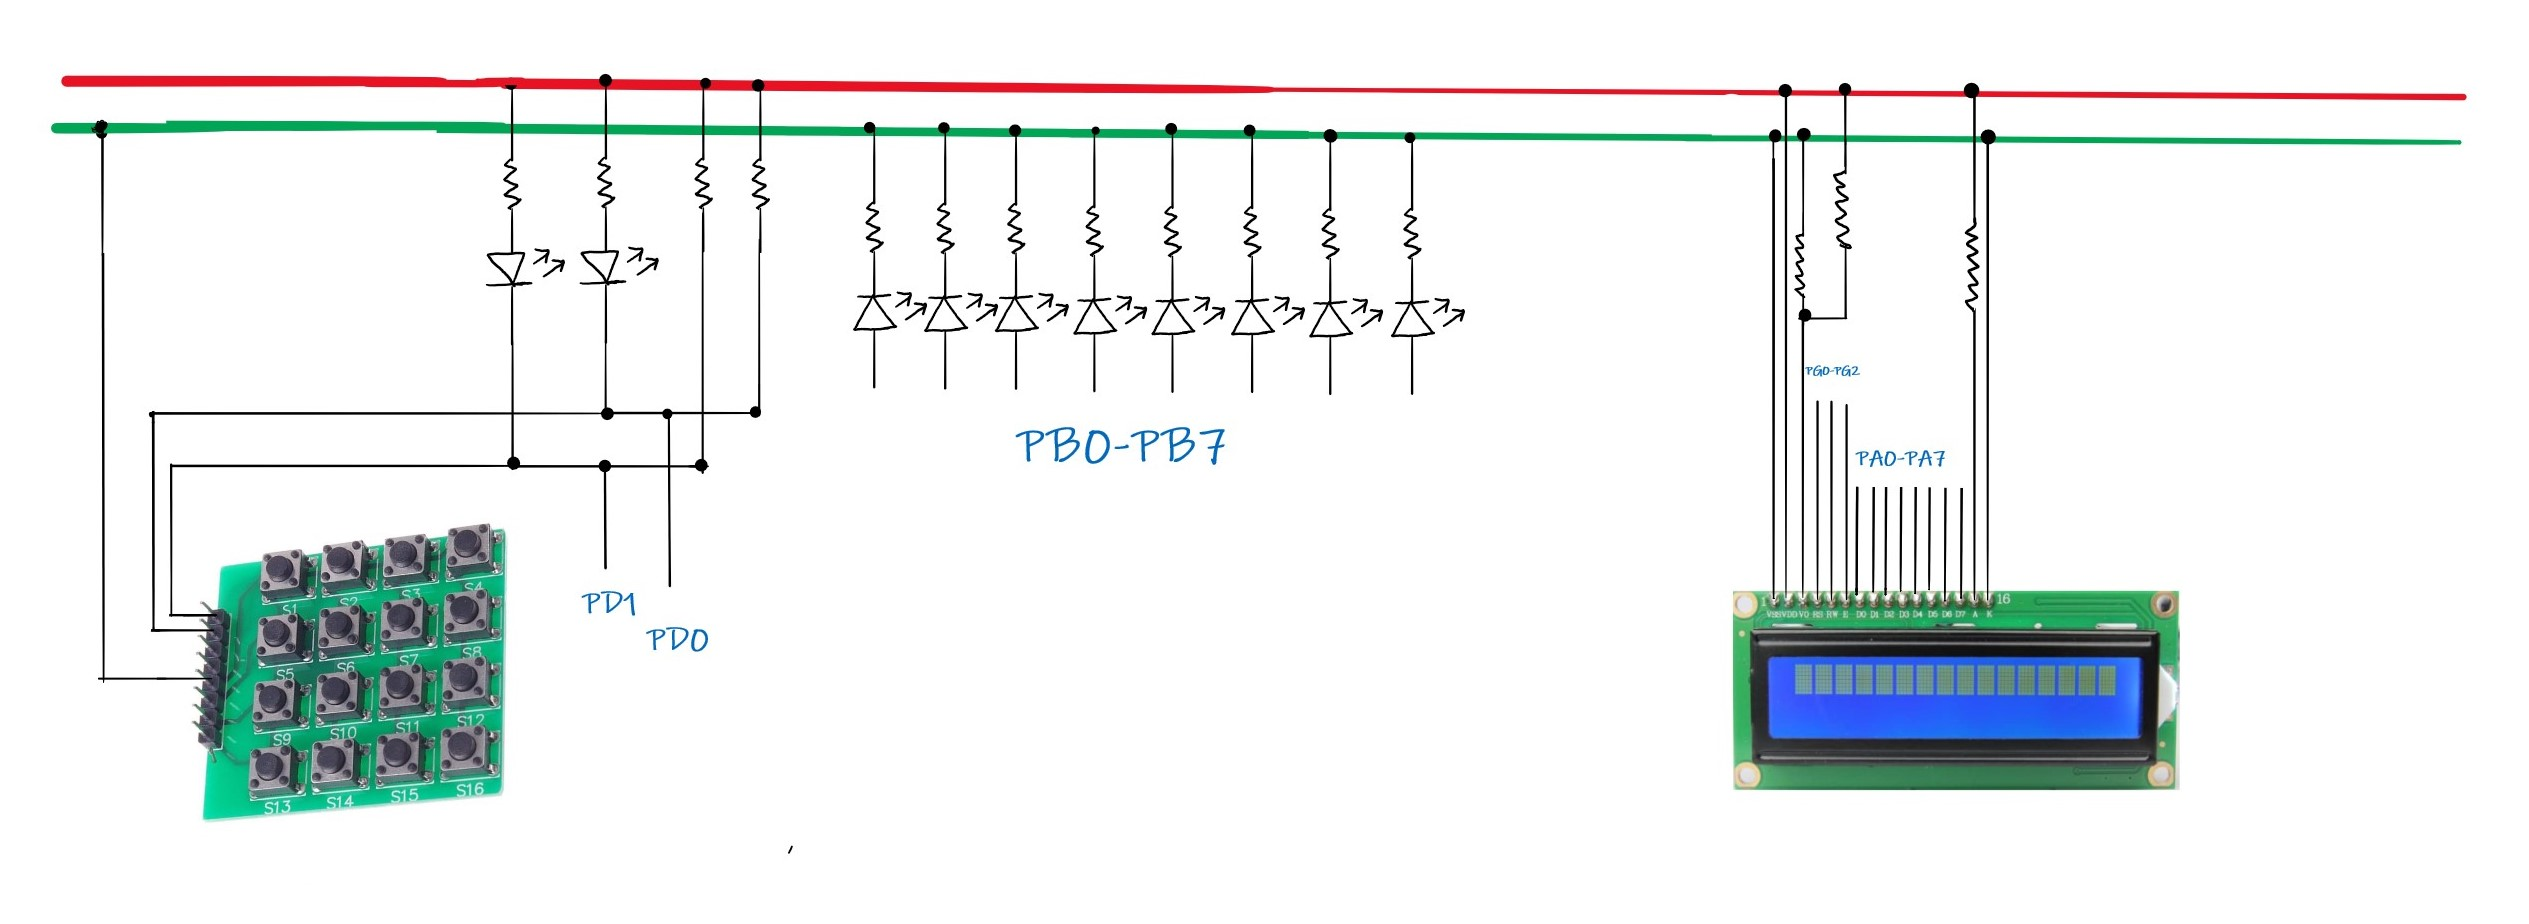
\includegraphics[width=1.1\linewidth,keepaspectratio]{slotschematic.jpg}
}
\caption{Circuit Diagram }
\label{Fig_Circuit_Diagram}
\end{figure}

\begin{figure}[h]
\centering{
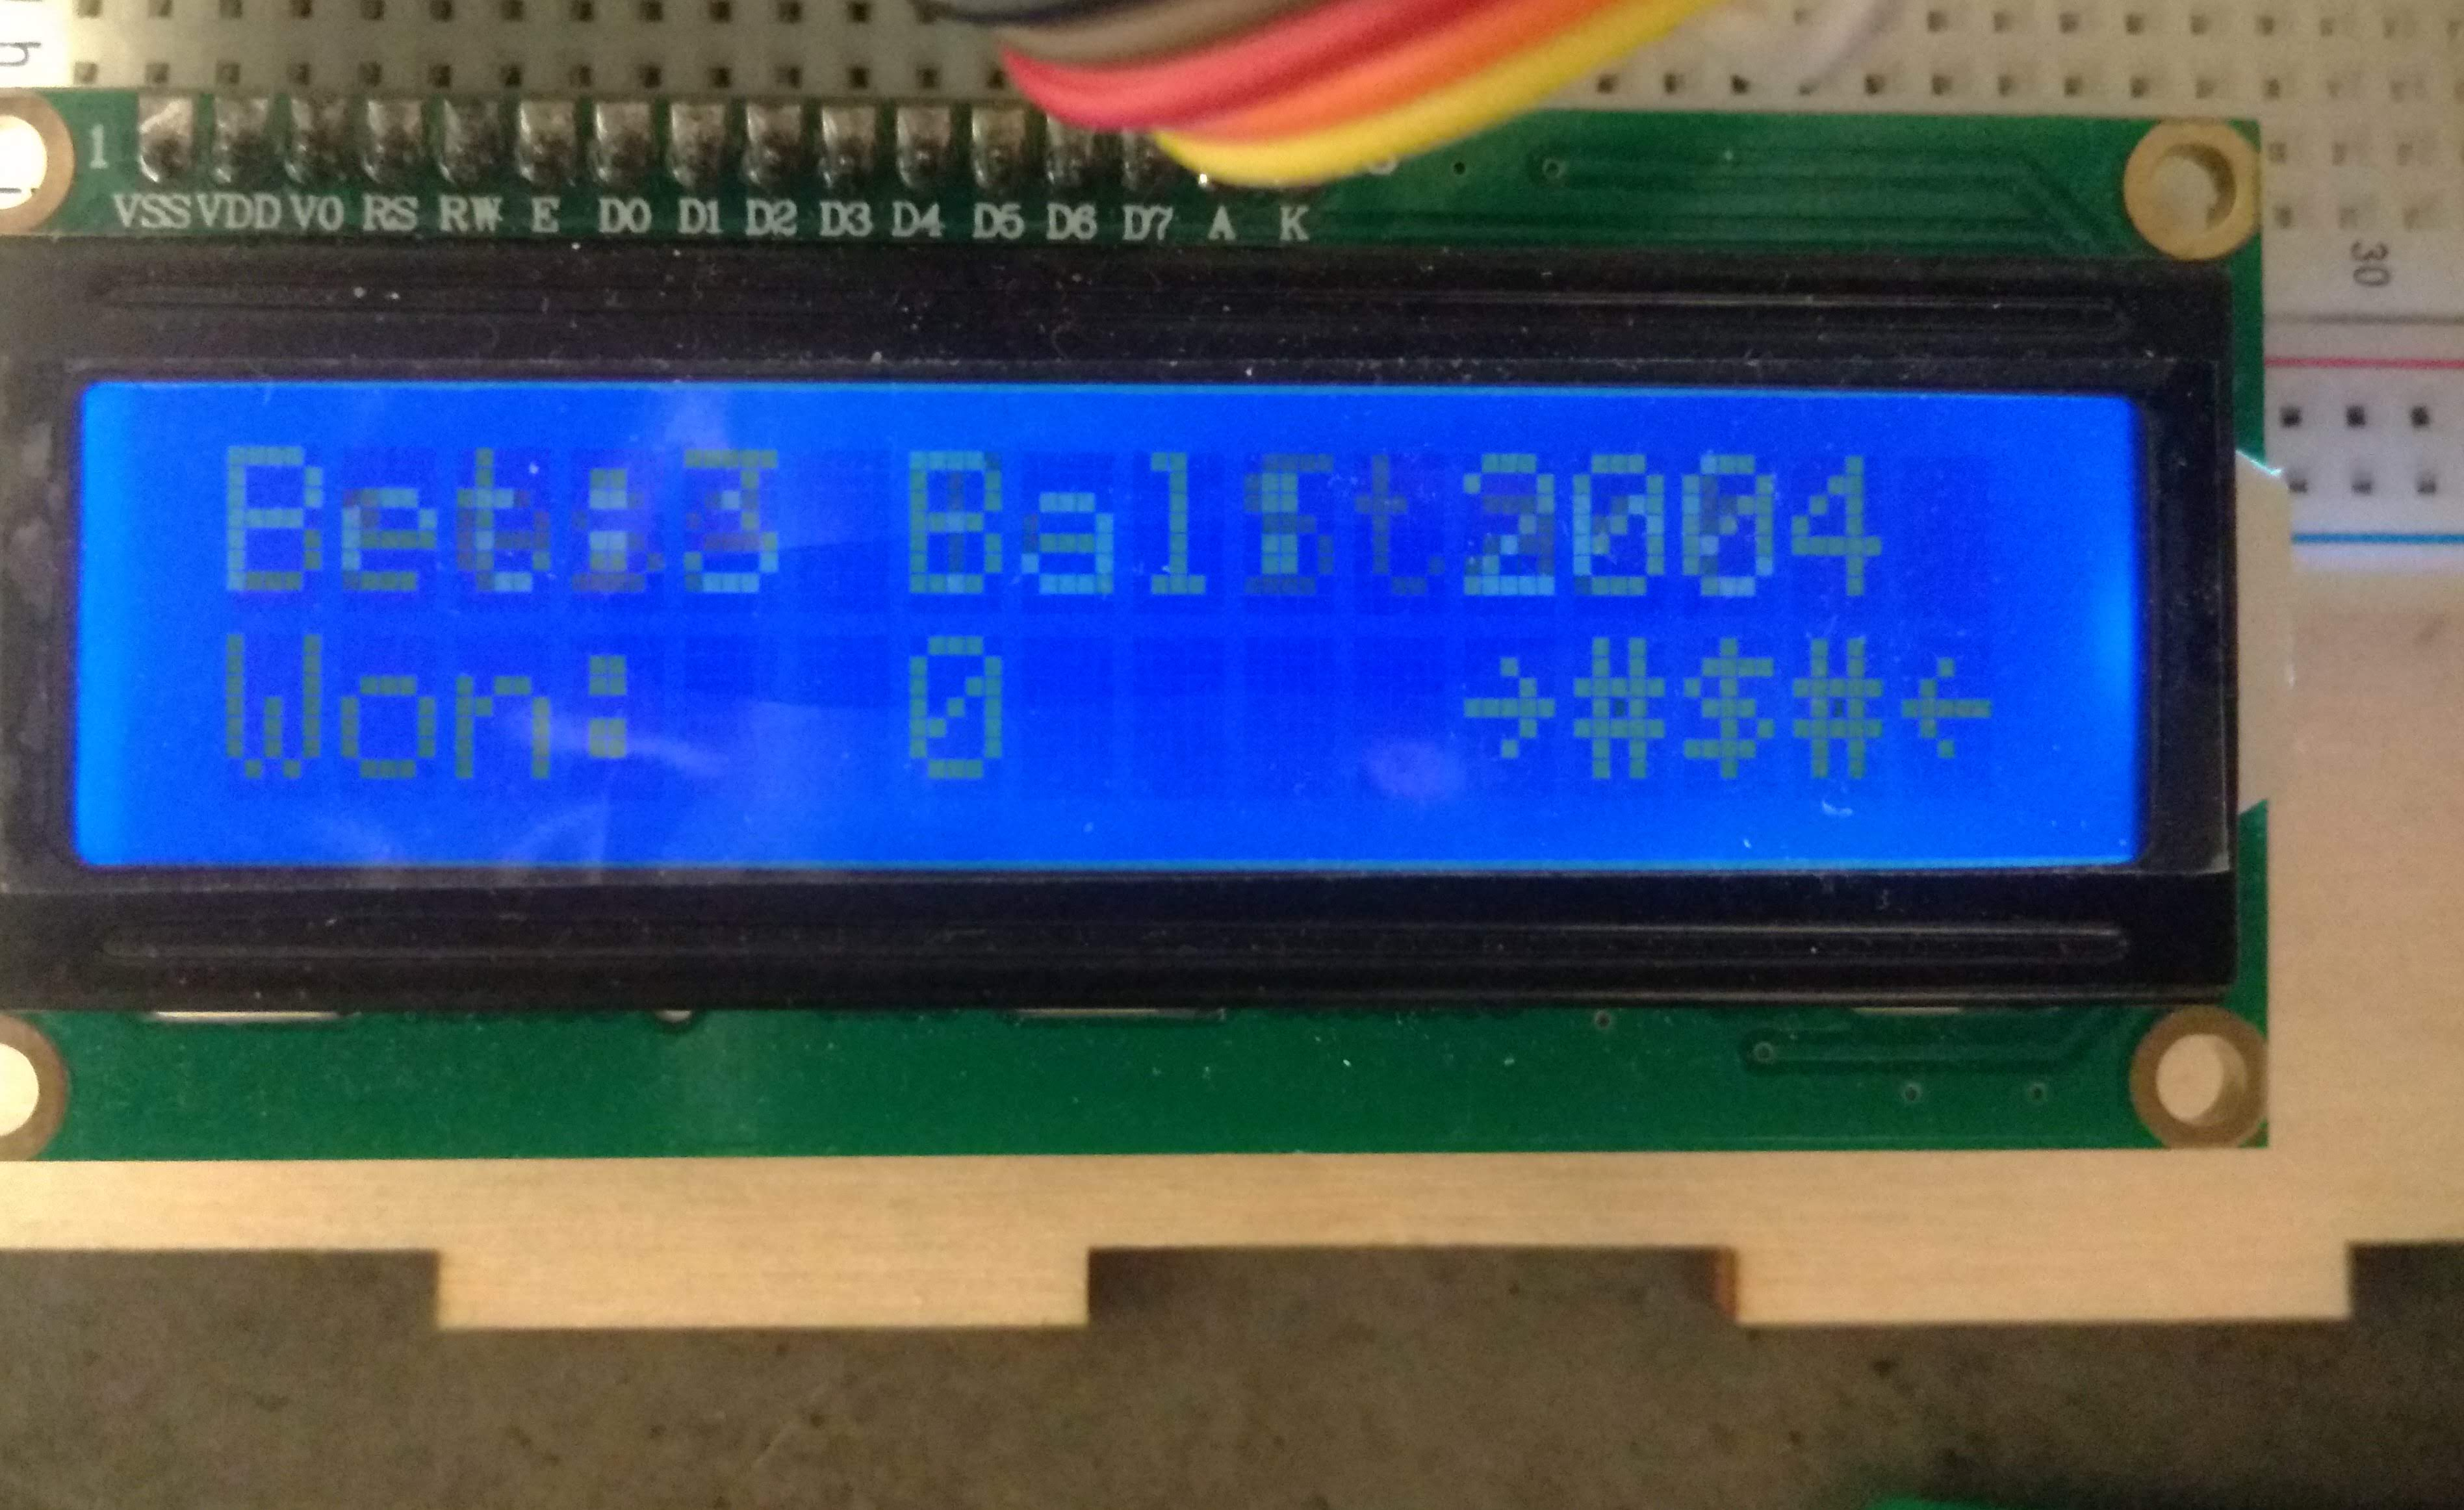
\includegraphics[width=\linewidth,keepaspectratio]{LCD_Slot_Machine.jpg}
}
\caption{LCD Display }
\label{Fig_LCD_Split}
\end{figure}
The life-size slot machine's spin and bet levers are realized by buttons. The life-size screen is realized by LCD. The LCD is divided into four sections:- bet section, balance section, winning amount section and wheel section. Figure \ref{Fig_LCD_Split} shows the division of section on LCD. The lighting effect is realized with 8 leds. The initial balance is set to 2000. Default bet value is 1. The three wheels of slot machine is represented by 3 led characters in the wheel section of LCD. Spin button is given higher priotity interrupt then the bet button. Timer 1 is used to check the activity time out. Activity time out is set to 15 seconds.  


\break
Timing requirements for the system are
\begin{itemize}
\item the response on button pressed should reflect on LCD within 1 sec.
\item the wheel spinning should not be so fast that the change of symbols on the screen is not obserable.
\item the wheel spinning should not be so slow that player gets enough time to stop by seeing symbol at screen.
\end{itemize}


\large \textbf{ Game Logic:}

\begin{itemize}
\item pressing bet button increases bet
\item pressing spin button toggles the spin functionality 
\item when spin is stopped and the wheels match the reward pattern, the balance is increased with reward
\item when spin is stopped and the wheels don't match the reward pattern, the bet value is deducted from balance
\item player wins the game, if the balance is reached to max value 10,000
\item player loses the game, if the balance becomes zero.
\end{itemize}

\large \textbf {Reward Patterns:}

\begin{itemize}
\item \normalsize \( \pi\ sym\ sym = bet * 5 \)   
\item \( \$ \$ \$ = bet * 10 \)  
\item \( Y Y Y = bet * 20  \)
\item \( \# \# \# = bet * 30 \) 
\item \tiny \( \sum \sum \sum\) \normalsize = bet * 50
\item \normalsize \( \pi \pi \pi = bet * 100 \)   
\end{itemize}
 




\chapter {Testing}
Black box and white box testing is done for the project. Codes were modified to replicate the desired testing scenarios. The list of test cases are listed below in tabular form.

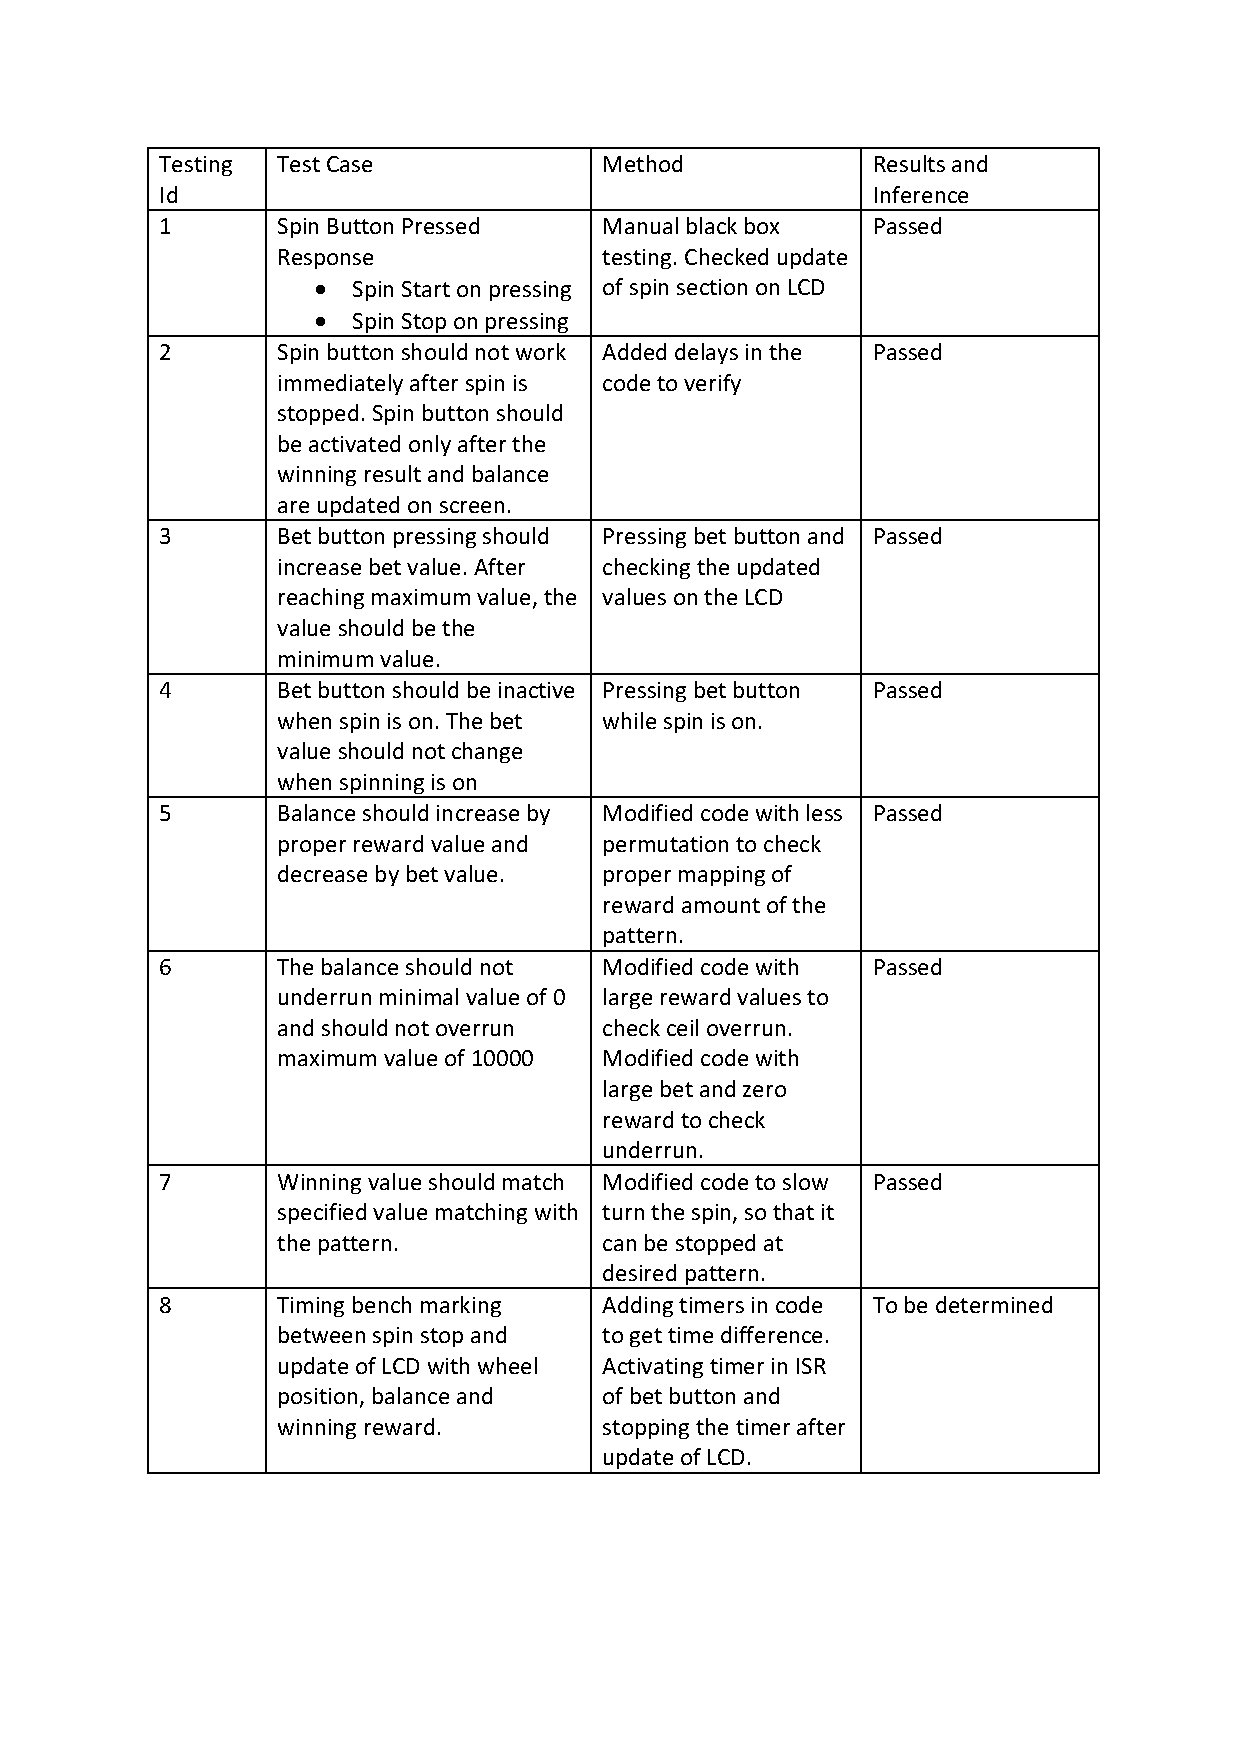
\includepdf[pages=-]{Testing_Matrix.pdf}

The Worst Case Execution Time WCET can be considered for the time of response when the spin is stopped and the values get updated. Consdering 1Mz clock speed, 37 \(\mu\)s write and command time for LCD, WCET can be calculated from code walkthrough. In function SM\_SpinWheel() in file SlotMachine.c, a while loop runs when spin is on, i.e. \textbf{while(SPIN\_ON == spinReels)}. It is considered the main routine is exactyly at this point when ISR routine for spin button is pressed. The longest code path till the LCD update occurs give the WCET. No reward pattern is considered for the longest code traversal. The calculated WCET rounds off to 104 ms.


\chapter {Source Listing}



\section{Config.h}
\begin{small}
\lstinputlisting[language=c,breaklines=true,numbers=left,tabsize=4]{../SlotMachineAtmelProject/SlotMachineAtmelProject/Config.h}
\end{small}

\section{LcdLibrary.h}
\begin{small}
\lstinputlisting[language=c,breaklines=true,numbers=left,tabsize=4]{../SlotMachineAtmelProject/SlotMachineAtmelProject/LcdLibrary.h}
\end{small}

\section{KeyPad.h}
\begin{small}
\lstinputlisting[language=c,breaklines=true,numbers=left,tabsize=4]{../SlotMachineAtmelProject/SlotMachineAtmelProject/KeyPad.h}
\end{small}

\section{SlotMachine.h}
\begin{small}
\lstinputlisting[language=c,breaklines=true,numbers=left,tabsize=4]{../SlotMachineAtmelProject/SlotMachineAtmelProject/SlotMachine.h}
\end{small}


\section{LcdLibrary.c}
\begin{small}
\lstinputlisting[language=c,breaklines=true,numbers=left,tabsize=4]{../SlotMachineAtmelProject/SlotMachineAtmelProject/LcdLibrary.c}
\end{small}


\section{KeyPad.c}
\begin{small}
\lstinputlisting[language=c,breaklines=true,numbers=left,tabsize=4]{../SlotMachineAtmelProject/SlotMachineAtmelProject/KeyPad.h}
\end{small}


\section{SlotMachine.c}
\begin{small}
\lstinputlisting[language=c,breaklines=true,numbers=left,tabsize=4]{../SlotMachineAtmelProject/SlotMachineAtmelProject/SlotMachine.c}
\end{small}


\section{Main.c}
\begin{small}
\lstinputlisting[language=c,breaklines=true,numbers=left,tabsize=4]{../SlotMachineAtmelProject/SlotMachineAtmelProject/Main.c}
\end{small}




\chapter {Critical evaluation and Conclusion}

\end{document}
